\section{Related Work}
\label{sec:related}

\noindent\textbf{Context Sensitivity in Tabular Foundation Models.}
Tabular foundation models predict unlabeled queries by conditioning on labeled
rows. TabPFN established synthetic-prior inference, TabICL extended tabular ICL
to larger datasets, and TabDPT combined retrieval with real-data
pretraining~\citep{muller2023tabpfn,qu2025tabicl,ma2025tabdpt}. Later variants
expanded pretraining, scalability, and task
coverage~\citep{hollmann2025tabpfn,grinsztajn2025tabpfn25,qu2026tabiclv2}.
Context-sampling studies further show that context size, coverage, and sampling
affect prediction accuracy and stability~\citep{abdullah2026contextsampling}.
These works improve model design and scale, but do not combine predictions from
differently constructed contexts under a frozen model.

\medskip
\noindent\textbf{Context Compression, Retrieval, and Selection.}
TuneTables, LoCalPFN, MixturePFN, and Tab-AICL construct inference contexts
through compression, retrieval, routing, or active acquisition,
respectively~\citep{feuer2024tunetables,thomas2024localpfn,xu2025mixturepfn,
treerath2026tabaicl}. \method{} extends context selection to context ensembling:
these methods optimize or select a dominant context or expert to improve
scalability or query relevance, whereas \method{} integrates predictions
induced by heterogeneous context constructors.

\medskip
\noindent\textbf{Context Ensembling and Construction Diversity.}
Beyond tabular learning, prior context ensembles combine predictions across
partitioned demonstration sets; DENSE, for example, averages their resulting
predictions~\citep{khalifa2023dense}. For tabular prediction, TabPFN ensembles
preprocessing and feature or label permutation
variants~\citep{hollmann2025tabpfn}. \method{} extends context ensembling from
variants of a shared construction scheme to heterogeneous constructors with
distinct inductive biases, assigning their influence from query-level evidence.

\begin{figure}[!t]
  \centering
  \ifdefined\ICLRLayout
  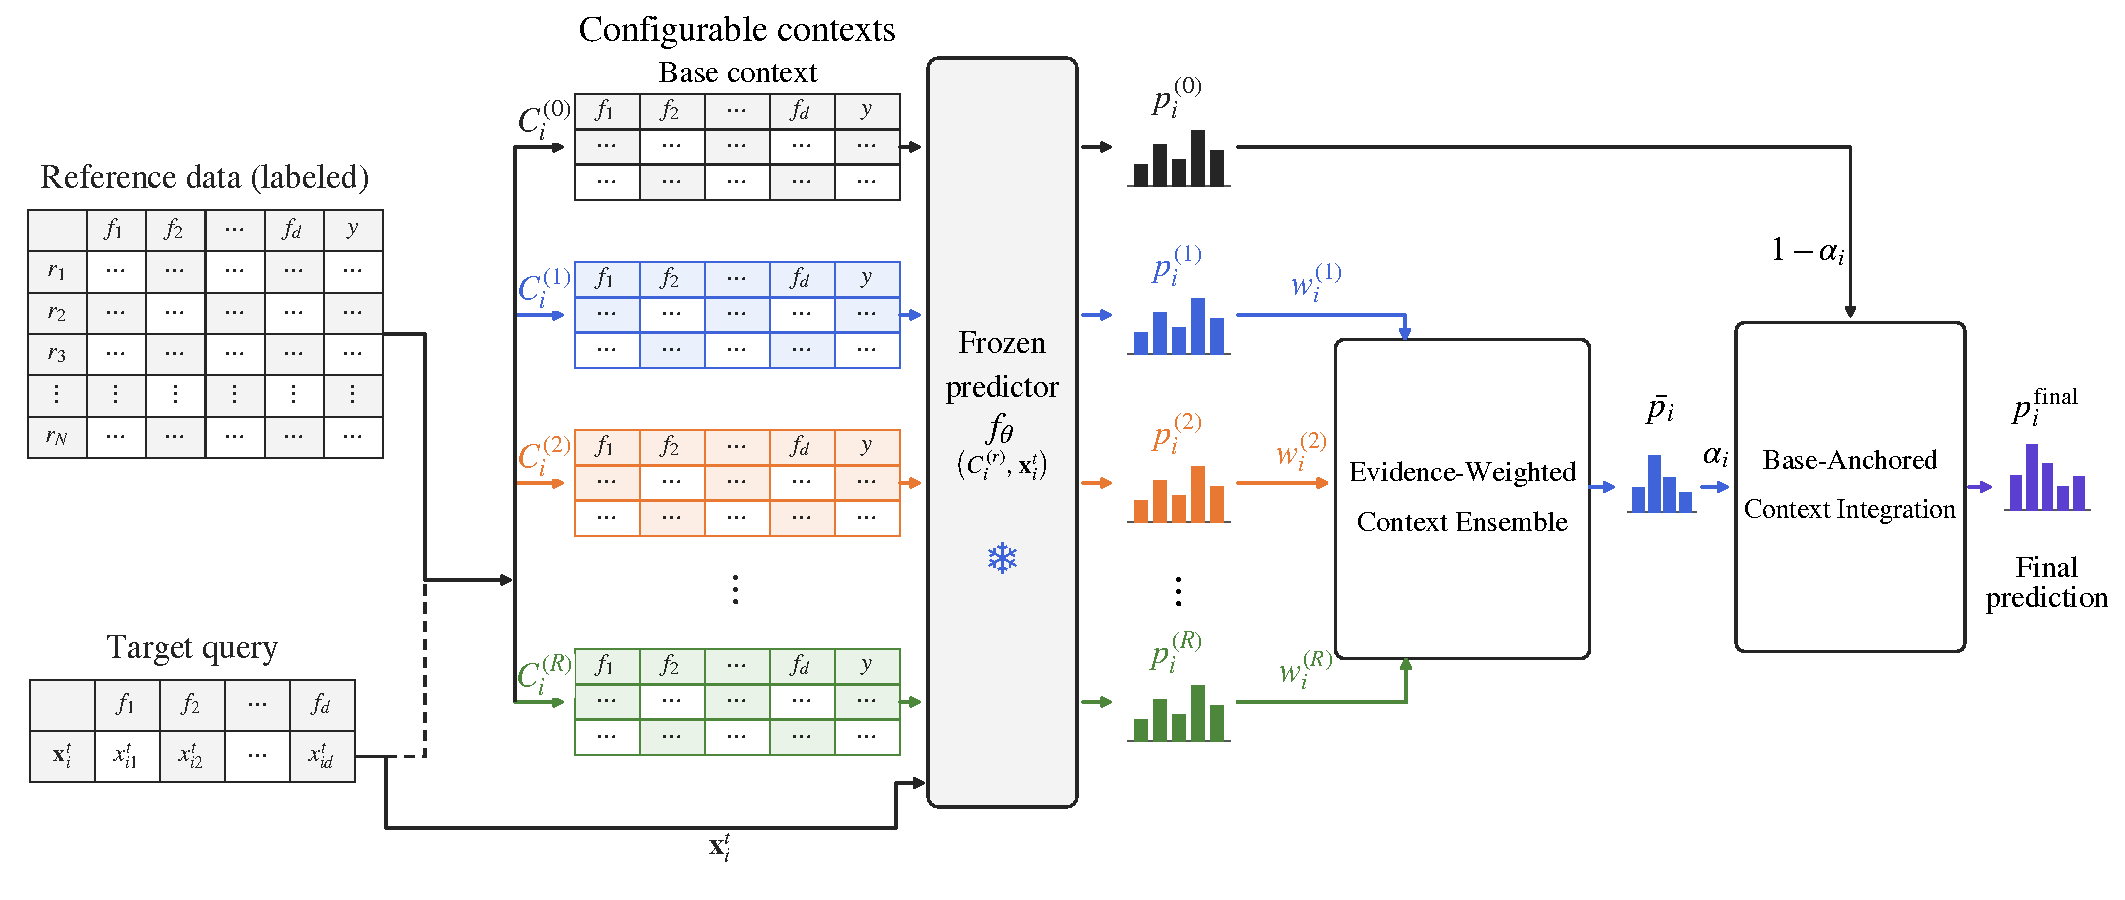
\includegraphics[width=\textwidth]{figures/context_ensemble_framework_pfn_input_semantics_fixed_lines.pdf}
  \else
    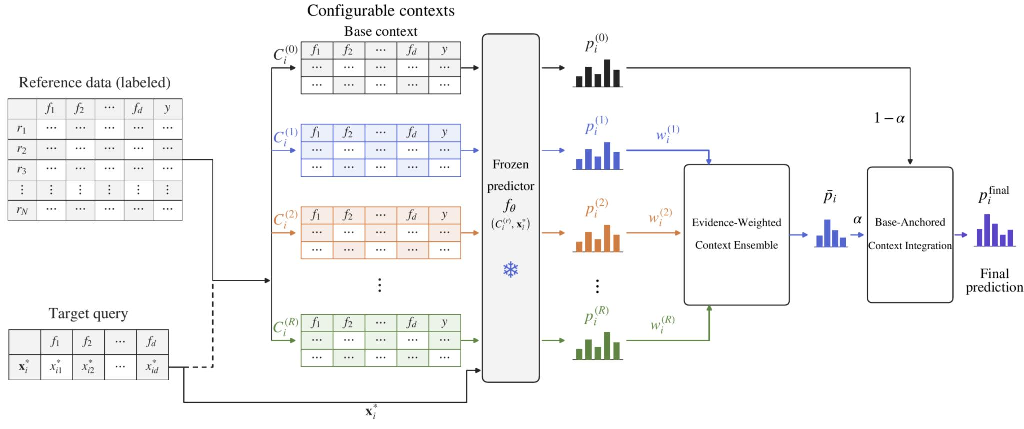
\includegraphics[width=0.86\textwidth]{figures/adaptive_context_ensemble_framework.pdf}
  \fi
  \caption{\textbf{Framework overview of \method{}.} For each query,
  configurable constructors form Base and alternative contexts evaluated by a
  frozen predictor. Evidence weighting aggregates the alternatives, and a
  Base-anchored gate blends the aggregate with Base into the final prediction.
  The shown $p_i^{(r)}$ are classification probability vectors; regression
  uses scalar $\hat y_i^{(r)}$ predictions in the same pipeline.}
  \label{fig:tabace_overview}
\end{figure}

\medskip
\noindent\textbf{Context Variability across Nominal and Shifted Conditions.}
Robust tabular prediction has been studied under several forms of data change.
Classical label-shift methods estimate or recalibrate target class
priors~\citep{lipton2018bbse,alexandari2020labelshift}, while DistPFN,
Drift-Resilient TabPFN, and SPN address label, temporal, and strategic shifts in
tabular ICL, respectively~\citep{lee2026distpfn,helli2024drifttabpfn,
lv2026strategic}. SkillTFM adapts frozen TFMs through evidence-conditioned
retrieval of external repair skills; a runtime certificate either admits a
repair or falls back to the base predictor~\citep{he2026skilltfm}. TableShift
and TabFSBench provide benchmarks for shifted
tabular tasks and controlled feature changes~\citep{gardner2023tableshift,
cheng2025tabfsbench}. Context-sampling results additionally show that context
choice affects TFM predictions under nominal
evaluation~\citep{abdullah2026contextsampling}. We therefore study context
aggregation under both nominal variability and multiple controlled change
families.
